\chapter{Leçon 22: Geometrie, Positiounen an nei Verben}

\section{Nei Verben / Nouveaux verbes / New verbs}

Dës Verbe si wichteg fir den Alldag. \textit{Ces verbes sont importants pour le quotidien. / These verbs are important for everyday life.}

\subsection*{Bleiwen (Rester / To stay)}
\begin{tabular}{ll c l l}
    \toprule
    \textbf{Pronom} & \textbf{Lëtzebuergesch} & \textbf{} & \textbf{Français} & \textbf{English} \\
    \midrule
    ech & bleiwen & $\rightarrow$ & Je reste & I stay \\
    du & bleifs & $\rightarrow$ & Tu restes & You stay \\
    hien / hatt / et & bleift & $\rightarrow$ & Il / Elle / On reste & He / She / It stays \\
    \midrule
    mir & bleiwen & $\rightarrow$ & Nous restons & We stay \\
    dir & bleift & $\rightarrow$ & Vous restez & You stay \\
    si & bleiwen & $\rightarrow$ & Ils / Elles restent & They stay \\
    \bottomrule
\end{tabular}
\\[1em]
\textbf{Imperativ:} Bleif! Bleift! (Reste ! Restez ! / Stay!)

\subsection*{Nodenken (Réfléchir / To think about)}
\begin{tabular}{ll c l l}
    \toprule
    \textbf{Pronom} & \textbf{Lëtzebuergesch} & \textbf{} & \textbf{Français} & \textbf{English} \\
    \midrule
    ech & denken no & $\rightarrow$ & Je réfléchis & I think \\
    du & denks no & $\rightarrow$ & Tu réfléchis & You think \\
    hien / hatt / et & denkt no & $\rightarrow$ & Il / Elle / On réfléchit & He / She / It thinks \\
    \midrule
    mir & denken no & $\rightarrow$ & Nous réfléchissons & We think \\
    dir & denkt no & $\rightarrow$ & Vous réfléchissez & You think \\
    si & denken no & $\rightarrow$ & Ils / Elles réfléchissent & They think \\
    \bottomrule
\end{tabular}
\\[1em]
\textbf{Imperativ:} Denk no! Denkt no! (Réfléchis ! Réfléchissez ! / Think! Think!)

\subsection*{Iwwerleeën (Réfléchir, considérer / To reflect, to consider)}
\textit{Synonym fir nodenken. / Synonyme de nodenken. / Synonym for nodenken.}
\\[0.5em]
\begin{tabular}{ll c l l}
    \toprule
    \textbf{Pronom} & \textbf{Lëtzebuergesch} & \textbf{} & \textbf{Français} & \textbf{English} \\
    \midrule
    ech & iwwerleeën & $\rightarrow$ & Je considère & I consider \\
    du & iwwerlees & $\rightarrow$ & Tu considères & You consider \\
    hien / hatt / et & iwwerleet & $\rightarrow$ & Il / Elle / On considère & He / She / It considers \\
    \midrule
    mir & iwwerleeën & $\rightarrow$ & Nous considérons & We consider \\
    dir & iwwerleet & $\rightarrow$ & Vous considérez & You consider \\
    si & iwwerleeën & $\rightarrow$ & Ils / Elles considèrent & They consider \\
    \bottomrule
\end{tabular}
\\[1em]
\textbf{Imperativ:} Iwwerlee! Iwwerleet! (Considère ! Considérez ! / Consider!)

\subsection*{Beschreiwen (Décrire / To describe)}
\begin{tabular}{ll c l l}
    \toprule
    \textbf{Pronom} & \textbf{Lëtzebuergesch} & \textbf{} & \textbf{Français} & \textbf{English} \\
    \midrule
    ech & beschreiwen & $\rightarrow$ & Je décris & I describe \\
    du & beschreifs & $\rightarrow$ & Tu décris & You describe \\
    hien / hatt / et & beschreift & $\rightarrow$ & Il / Elle / On décrit & He / She / It describes \\
    \midrule
    mir & beschreiwen & $\rightarrow$ & Nous décrivons & We describe \\
    dir & beschreift & $\rightarrow$ & Vous décrivez & You describe \\
    si & beschreiwen & $\rightarrow$ & Ils / Elles décrivent & They describe \\
    \bottomrule
\end{tabular}
\\[1em]
\textbf{Imperativ:} Beschreif! Beschreift! (Décris ! Décrivez ! / Describe!)

\subsection*{Molen (Dessiner, peindre / To draw, to paint)}
\begin{tabular}{ll c l l}
    \toprule
    \textbf{Pronom} & \textbf{Lëtzebuergesch} & \textbf{} & \textbf{Français} & \textbf{English} \\
    \midrule
    ech & molen & $\rightarrow$ & Je dessine & I draw \\
    du & mols & $\rightarrow$ & Tu dessines & You draw \\
    hien / hatt / et & molt & $\rightarrow$ & Il / Elle / On dessine & He / She / It draws \\
    \midrule
    mir & molen & $\rightarrow$ & Nous dessinons & We draw \\
    dir & molt & $\rightarrow$ & Vous dessinez & You draw \\
    si & molen & $\rightarrow$ & Ils / Elles dessinent & They draw \\
    \bottomrule
\end{tabular}
\\[1em]
\textbf{Imperativ:} Mol! Molt! (Dessine ! Dessinez ! / Draw!)

\vspace{1cm}

\section{Geometresch Figuren / Figures géométriques / Geometric figures}

\begin{center}
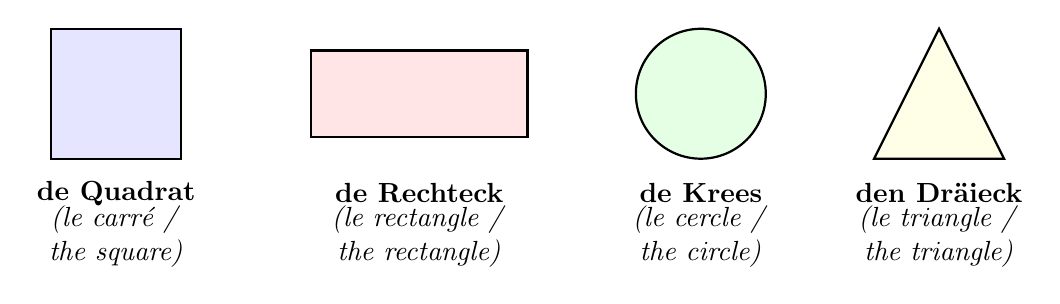
\begin{tikzpicture}[scale=1.1]
    % Quadrat
    \draw[thick, fill=blue!10] (0,0) rectangle (1.5,1.5);
    \node at (0.75, -0.4) {\textbf{de Quadrat}};
    \node[align=center] at (0.75, -0.9) {\textit{(le carré /} \\ \textit{the square)}};
    
    % Rechteck
    \draw[thick, fill=red!10] (3,0.25) rectangle (5.5,1.25);
    \node at (4.25, -0.4) {\textbf{de Rechteck}};
    \node[align=center] at (4.25, -0.9) {\textit{(le rectangle /} \\ \textit{the rectangle)}};
    
    % Krees
    \draw[thick, fill=green!10] (7.5,0.75) circle (0.75);
    \node at (7.5, -0.4) {\textbf{de Krees}};
    \node[align=center] at (7.5, -0.9) {\textit{(le cercle /} \\ \textit{the circle)}};
    
    % Dräieck
    \draw[thick, fill=yellow!10] (9.5,0) -- (11,0) -- (10.25, 1.5) -- cycle;
    \node at (10.25, -0.4) {\textbf{den Dräieck}};
    \node[align=center] at (10.25, -0.9) {\textit{(le triangle /} \\ \textit{the triangle)}};
\end{tikzpicture}
\end{center}

\vspace{1cm}

\section{Positiounen an Direktiounen / Positions et Directions / Positions and Directions}

Hei si vill wichteg Wierder fir Positiounen ze beschreiwen. \textit{Voici beaucoup de mots importants pour décrire des positions. / Here are many important words to describe positions.}

\subsection*{Uewen vs. Ënnen}
\begin{itemize}
    \item \textbf{Uewen:} En haut / Above, up. (e.g. \textit{D'Buch ass uewen um Regal. / Le livre est en haut sur l'étagère. / The book is high up on the shelf.})
    \item \textbf{Ënnen:} En bas / Below, down. (e.g. \textit{De Ball ass ënnen. / Le ballon est en bas. / The ball is down below.})
\end{itemize}

\subsection*{Uewendrop vs. Ënnendrënner}
\begin{itemize}
    \item \textbf{Uewendrop:} Par-dessus, au-dessus / On top of, over. (e.g. \textit{Uewendrop leie Saachen. / Des choses sont posées par-dessus. / Things are lying on top.})
    \item \textbf{Ënnendrënner:} En dessous, par en dessous / Underneath, below. (e.g. \textit{Eppes läit ënnendrënner. / Quelque chose est posé en dessous. / Something is lying underneath.})
    \item \textit{Bemierkung:} "Uewendrop" gëtt benotzt, wann eppes direkt op enger Uewerfläch läit. "Uewendriwwer" heescht "au-dessus", dacks mat Ofstand. \textit{(Remarque : "Uewendrop" est utilisé quand quelque chose repose directement sur une surface, "on top of". "Uewendriwwer" signifie au-dessus, souvent avec une distance, "above". / Note: "Uewendrop" is used when something lies directly on a surface, "on top of". "Uewendriwwer" means above, often with a gap, "above".)}
\end{itemize}

\subsection*{Virun vs. Virdrun (Zäit an Uert / Temps et Lieu / Time and Place)}
\begin{itemize}
    \item \textbf{Virun:} Devant (lieu) ou il y a (temps) / In front of (place) or ago (time). 
        \begin{itemize}
            \item \textit{Ech hunn hie virum Haus gesinn. / Je l'ai vu devant la maison. / I saw him in front of the house.} (Lieu / Place)
            \item \textit{Ech hunn hie viru 4 Deeg gesinn. / Je l'ai vu il y a 4 jours. / I saw him 4 days ago.} (Zäit / Time)
        \end{itemize}
    \item \textbf{Virdrun:} Avant, auparavant (temps) ou devant, à l'avant (lieu) / Before, beforehand (time) or in front (place). 
        \begin{itemize}
            \item \textit{Ech hunn hie virdrun gesinn. / Je l'ai vu avant. / I saw him before.} (Zäit / Time)
            \item \textit{Hei ass de Paul, an d'Anne steet virdrun. / Voici Paul, et Anne se tient devant. / Here is Paul, and Anne stands before him.} (Lieu / Place)
        \end{itemize}
\end{itemize}

\subsection*{Lénks, Riets an Niewent}
\begin{itemize}
    \item \textbf{Lénks vum / Op der lénker Säit:} À gauche de / sur le côté gauche / To the left of / on the left side.
        \begin{itemize}
            \item \textit{De Buttek ass lénks vum Haus. / Le magasin est à gauche de la maison. / The shop is to the left of the house.}
        \end{itemize}
    \item \textbf{Riets vum / Op der rietser Säit:} À droite de / sur le côté droit / To the right of / on the right side.
        \begin{itemize}
            \item \textit{De Bam ass riets vum Auto. / L'arbre est à droite de la voiture. / The tree is to the right of the car.}
        \end{itemize}
    \item \textbf{Nieft / Niewent / Niewen:} À côté de / Next to, beside.
        \begin{itemize}
            \item \textit{Ech sëtzen niewent mengem Frënd. / Je suis assis à côté de mon ami. / I am sitting next to my friend.}
        \end{itemize}
    \item \textbf{Ronderëm:} Autour de / Around.
    \item \textbf{Vis-à-vis:} En face de / Opposite.
\end{itemize}

\subsection*{Ënnert vs. Iwwert (Sous vs. Au-dessus / Under vs. Over)}
Mat dëse Wierder benotze mir den Dativ: \textbf{dem} (m/n), \textbf{der} (f), \textbf{den} (pl). \textit{(Avec ces mots nous utilisons le datif. / With these words we use the dative.)}
\begin{itemize}
    \item \textbf{Ënnert dem / ënnert der / ënnert den:} Sous le/la/les / Under the.
        \begin{itemize}
            \item \textit{De Ball ass ënnert dem Kartong (m).} (Le ballon est sous le carton. / The ball is under the box.)
        \end{itemize}
    \item \textbf{Iwwert dem / iwwert der / iwwert den:} Au-dessus de / Over, above.
        \begin{itemize}
            \item \textit{D'Luucht hänkt iwwert dem Dësch (m).} (La lampe est suspendue au-dessus de la table. / The lamp hangs over the table.)
        \end{itemize}
\end{itemize}
\textit{Bemierkung: Ënnen ass d'Richtung, ënnert dem heescht ënnert engem Objet. (Remarque : "Ënnen" est la direction, "ënnert dem" signifie sous un objet. / Note: "Ënnen" is the direction (down), "ënnert dem" means under an object.)}

\subsection*{Hannert vs. Virun (Derrière vs. Devant / Behind vs. In front of)}
\begin{itemize}
    \item \textbf{Hannert dem / hannert der / hannert den:} Derrière le/la/les / Behind the.
        \begin{itemize}
            \item \textit{Hannert dem Haus (n) ass e Gaart.} (Derrière la maison il y a un jardin. / Behind the house there is a garden.)
        \end{itemize}
    \item \textbf{Virum (virun dem) / virun der / virun den:} Devant le/la/les / In front of the.
        \begin{itemize}
            \item \textit{Den Auto steet virum Haus (n).} (La voiture se trouve devant la maison. / The car is parked in front of the house.)
        \end{itemize}
\end{itemize}

\vspace{1cm}

\section{Positiounsverben / Verbes de Position / Verbs of Position}

Lëtzebuergesch mécht en Ënnerscheed tëscht \textbf{Aktioun} (mouvement) an \textbf{Zoustand} (état, position). \textit{Le luxembourgeois fait une différence entre action et état. / Luxembourgish distinguishes between action and state.}

\subsection*{1. Sëtzen vs. Setzen (Assis vs. Asseoir / Sitting vs. To sit down)}
\begin{itemize}
    \item \textbf{Sëtzen (Zoustand / État / State):} Être assis / To be sitting.
        \begin{itemize}
            \item \textit{Ech sëtze schonn.} (Je suis déjà assis. / I am already sitting.)
        \end{itemize}
    \item \textbf{Setzen (Aktioun / Action):} S'asseoir, poser / To sit down, to place.
        \begin{itemize}
            \item \textit{Ech setze mech.} (Je m'assieds. / I sit down.)
        \end{itemize}
\end{itemize}

\textbf{Ausdréck an Nuancen mat Sëtzen:}
\begin{itemize}
    \item \textbf{Dir sëtzt um Dësch.} (Vous êtes assis à la table / You are sitting at the table). \\ \textit{Bemierkung: "um" ka fir "op dem" oder "un dem" stoen. (Remarque : "um" peut vouloir dire "op dem" [sur le] ou "un dem" [au]. / Note: "um" can stand for "op dem" [on the] or "un dem" [at the].)}
    \item \textbf{Du sëtzt beim Dësch.} (Tu es assis près de la table / You are sitting by the table).
    \item \textbf{Mir sëtze ronderëm den Dësch.} (Nous sommes assis autour de la table / We are sitting around the table).
    \item \textbf{Figurativ:} \textit{Hie sëtzt op sengem Geld.} [Hien ass ganz knéckeg] (Il est assis sur son argent. [Il est très radin] / He sits on his money. [He is very stingy]).
    \item \textbf{Figurativ:} \textit{Hie sëtzt elo.} (Il est en prison. / He is in prison now).
\end{itemize}

\begin{center}
    \begin{minipage}[t]{0.45\textwidth}
        \centering
        
\includegraphics[width=0.8\linewidth]{vokab_300dpi/s_tzen_un.png} \\
        \textit{Hie sëtzt un dem Dësch (um Dësch). \\ (Il est assis à la table / He sits at the table.)}
    \end{minipage}
    \hfill
    \begin{minipage}[t]{0.45\textwidth}
        \centering
        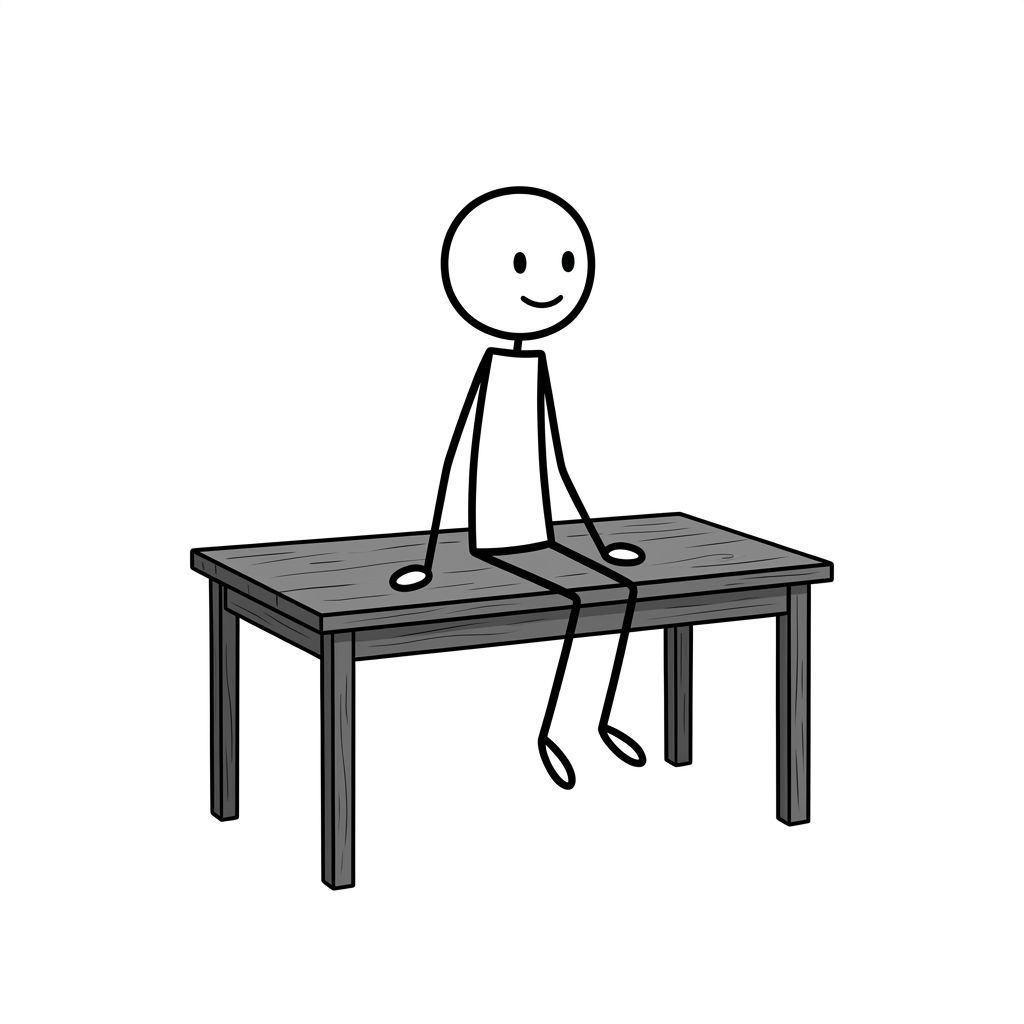
\includegraphics[width=0.8\linewidth]{vokab_300dpi/s_tzen_op.png} \\
        \textit{Hie sëtzt op dem Dësch (um Dësch). \\ (Il est assis sur la table / He sits on the table.)}
    \end{minipage}
\end{center}

\subsection*{2. Stoen vs. Stellen (Debout vs. Placer / Standing vs. To put standing)}
\begin{itemize}
    \item \textbf{Stoen (Zoustand):} Être debout / To stand, to be standing.
    \item \textbf{Stellen (Aktioun):} Placer, poser debout / To put, to place upright.
\end{itemize}

\textbf{Ausdréck mat Stoen:}
\begin{itemize}
    \item \textbf{Ech stinn op.} (Je me lève. / I stand up - \textit{Exception: here it is an action}).
    \item \textbf{Elo stinn ech do.} (Maintenant je me tiens là. / Now I stand there).
    \item \textbf{Stéi riicht! / Stitt riicht!} (Tiens-toi droit ! / Tenez-vous droit ! / Stand up straight!).
    \item \textbf{Stéi op, et ass Zäit / et gëtt Zäit.} (Lève-toi, il est temps. / Get up, it's time).
    \item \textbf{Ech stinn dozou!} (J'assume ! / I stand by it!).
    \item \textbf{Ech stinn zu mengem Frënd.} (Je soutiens mon ami. / I stand by my friend).
\end{itemize}

\subsection*{3. Leien vs. Leeën (Couché vs. Coucher / Lying down vs. To lay down)}
\begin{itemize}
    \item \textbf{Leien (Zoustand):} Être couché / To lie, to be lying down.
    \item \textbf{Leeën (Aktioun):} Coucher, poser à plat / To lay down, to place flat.
\end{itemize}

\subsection*{Stoen / Leien vs. Sinn}
Heiansdo kann ee \textbf{sinn} benotzen amplaz vu stoen oder leien. \textit{Parfois on peut utiliser "sinn" au lieu de "stoen" ou "leien". / Sometimes one can use "sinn" instead of "stoen" or "leien".}
\begin{itemize}
    \item \textbf{Ech stinn do} vs \textbf{Ech sinn do.} (Je me tiens là vs Je suis là / I stand there vs I am there).
    \item \textbf{D'Iessen steet um Dësch} vs \textbf{D'Iessen ass um Dësch.} (La nourriture est posée sur la table vs La nourriture est sur la table / The food is on the table).
\end{itemize}

\vspace{1cm}

\section{Aner Wierder / Autres mots / Other words}

\begin{itemize}
    \item \textbf{Generéis / Mëtschgieweg:} Généreux / Generous. (\textit{Mëtschgieweg} ass de Lëtzebuerger Begrëff / le terme luxembourgeois / the Luxembourgish term).
    \item \textbf{D'Mëntz:} La monnaie (pièces) / The coin, the change.
    \item \textbf{De Fric:} Le fric, l'argent (familier) / The dough, cash (slang).
\end{itemize}

\vspace{1.5cm}
\color{geminiBlue}\hrule height 1.5pt \vspace{0.5em}\color{black}
\section[Vokabulär: Bau an Elektresch]{Vokabulär: Bau an Elektresch / Construction et Électricité / Construction and Electricity}

\begin{itemize}
    \item \textbf{de Kartong / de Kartrong} (Pl.: d'Kartongen) $\rightarrow$ un carton (a cardboard box)
    \item \textbf{d'Schinn} (Pl.: d'Schinnen) $\rightarrow$ un rail (a rail/track)
    \item \textbf{d'Leitung} (Pl.: d'Leitungen) $\rightarrow$ un câble, une conduite (a cable/wire, a pipe)
\end{itemize}

\vspace{1em}

\begin{center}
    \begin{minipage}[t]{0.3\textwidth}
        \centering
        \textbf{E Kartong}
        \vspace{0.5em}
        \framebox{\parbox{0.9\linewidth}{\centering
            \vspace{0.5cm}
            
\includegraphics[width=0.9\linewidth]{vokab_300dpi/kartong.png} \\
            \small\textit{De Kartong (Le carton / The box)}
            \vspace{0.5cm}
        }}
    \end{minipage}
    \hfill
    \begin{minipage}[t]{0.3\textwidth}
        \centering
        \textbf{Eng Schinn}
        \vspace{0.5em}
        \framebox{\parbox{0.9\linewidth}{\centering
            \vspace{0.5cm}
            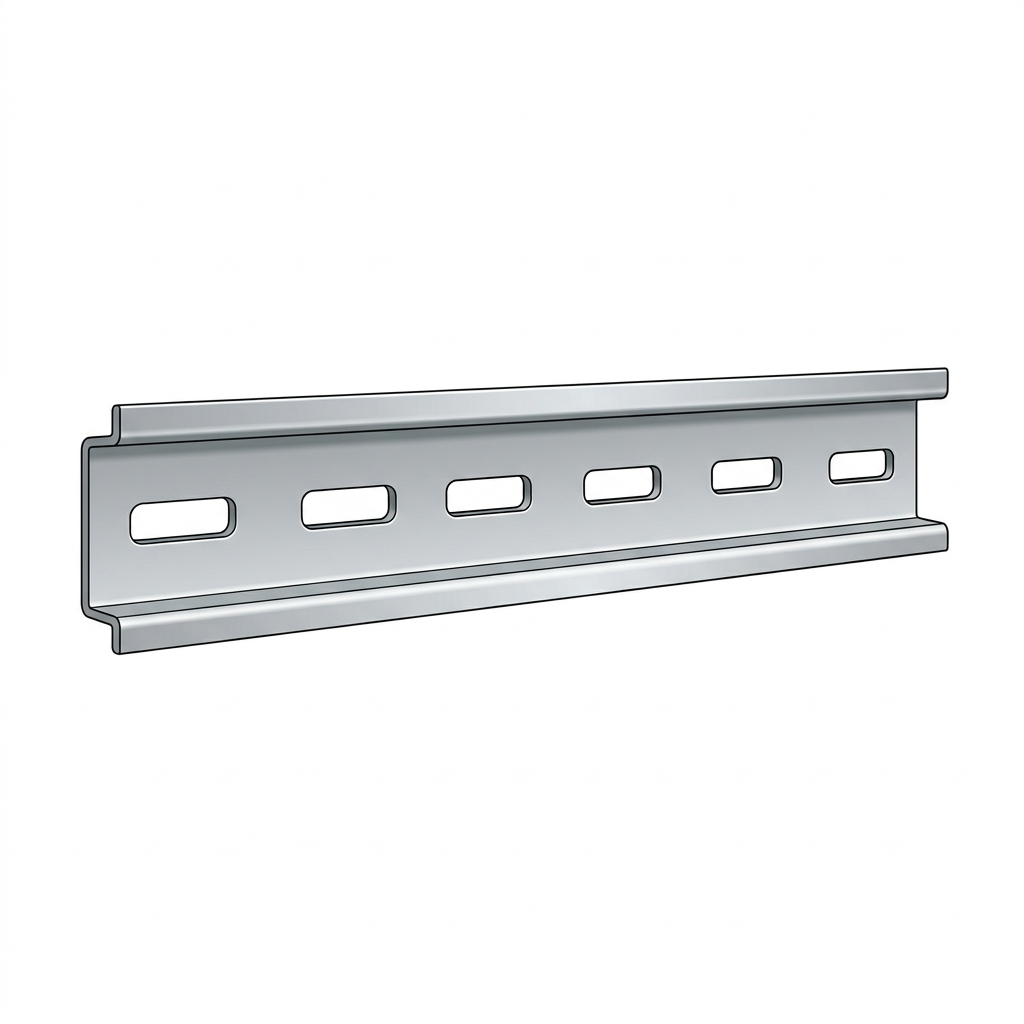
\includegraphics[width=0.9\linewidth]{vokab_300dpi/schinn.png} \\
            \small\textit{D'Schinn (Le rail / The rail)}
            \vspace{0.5cm}
        }}
    \end{minipage}
    \hfill
    \begin{minipage}[t]{0.3\textwidth}
        \centering
        \textbf{Eng Leitung}
        \vspace{0.5em}
        \framebox{\parbox{0.9\linewidth}{\centering
            \vspace{0.5cm}
            
\includegraphics[width=0.9\linewidth]{vokab_300dpi/leitung.png} \\
            \small\textit{D'Leitung (Le câble / The cable)}
            \vspace{0.5cm}
        }}
    \end{minipage}
\end{center}
